% Section content template for individual Educative lessons
% This file contains the actual content for a specific section
% Generated from Educative API section content

% Section: SOLID: Liskov Substitution Principle
% Section ID: 4941477451137024
% Section Slug: solid-liskov-substitution-principle
% Generated: 2025-12-11T05:50:20.914813

\subsection{\texorpdfstring{Introduction\href{https://www.educative.io/pageeditor/10370001/5583710957338624/6062503710949376\#Introduction}{}}{Introduction}}\label{introduction}
\\
The \textbf{Liskov Substitution Principle (LSP)} is one of the fundamental design principles of object-oriented design. The LSP helps guide the use of inheritance in design so that the application does not break. It states that the objects of a subclass should behave the same way as the objects of the superclass, such that they are replaceable. This rule generally applies to abstraction concepts like inheritance and polymorphism.

\subsection{The Vehicle class}\label{the-vehicle-class}
\\
Let\textquotesingle s construct a simple class called \texttt{Vehicle} that has some attributes and methods and a subclass \texttt{Car} that extends it as shown below:

\begin{figure}[htbp]
 \centering
 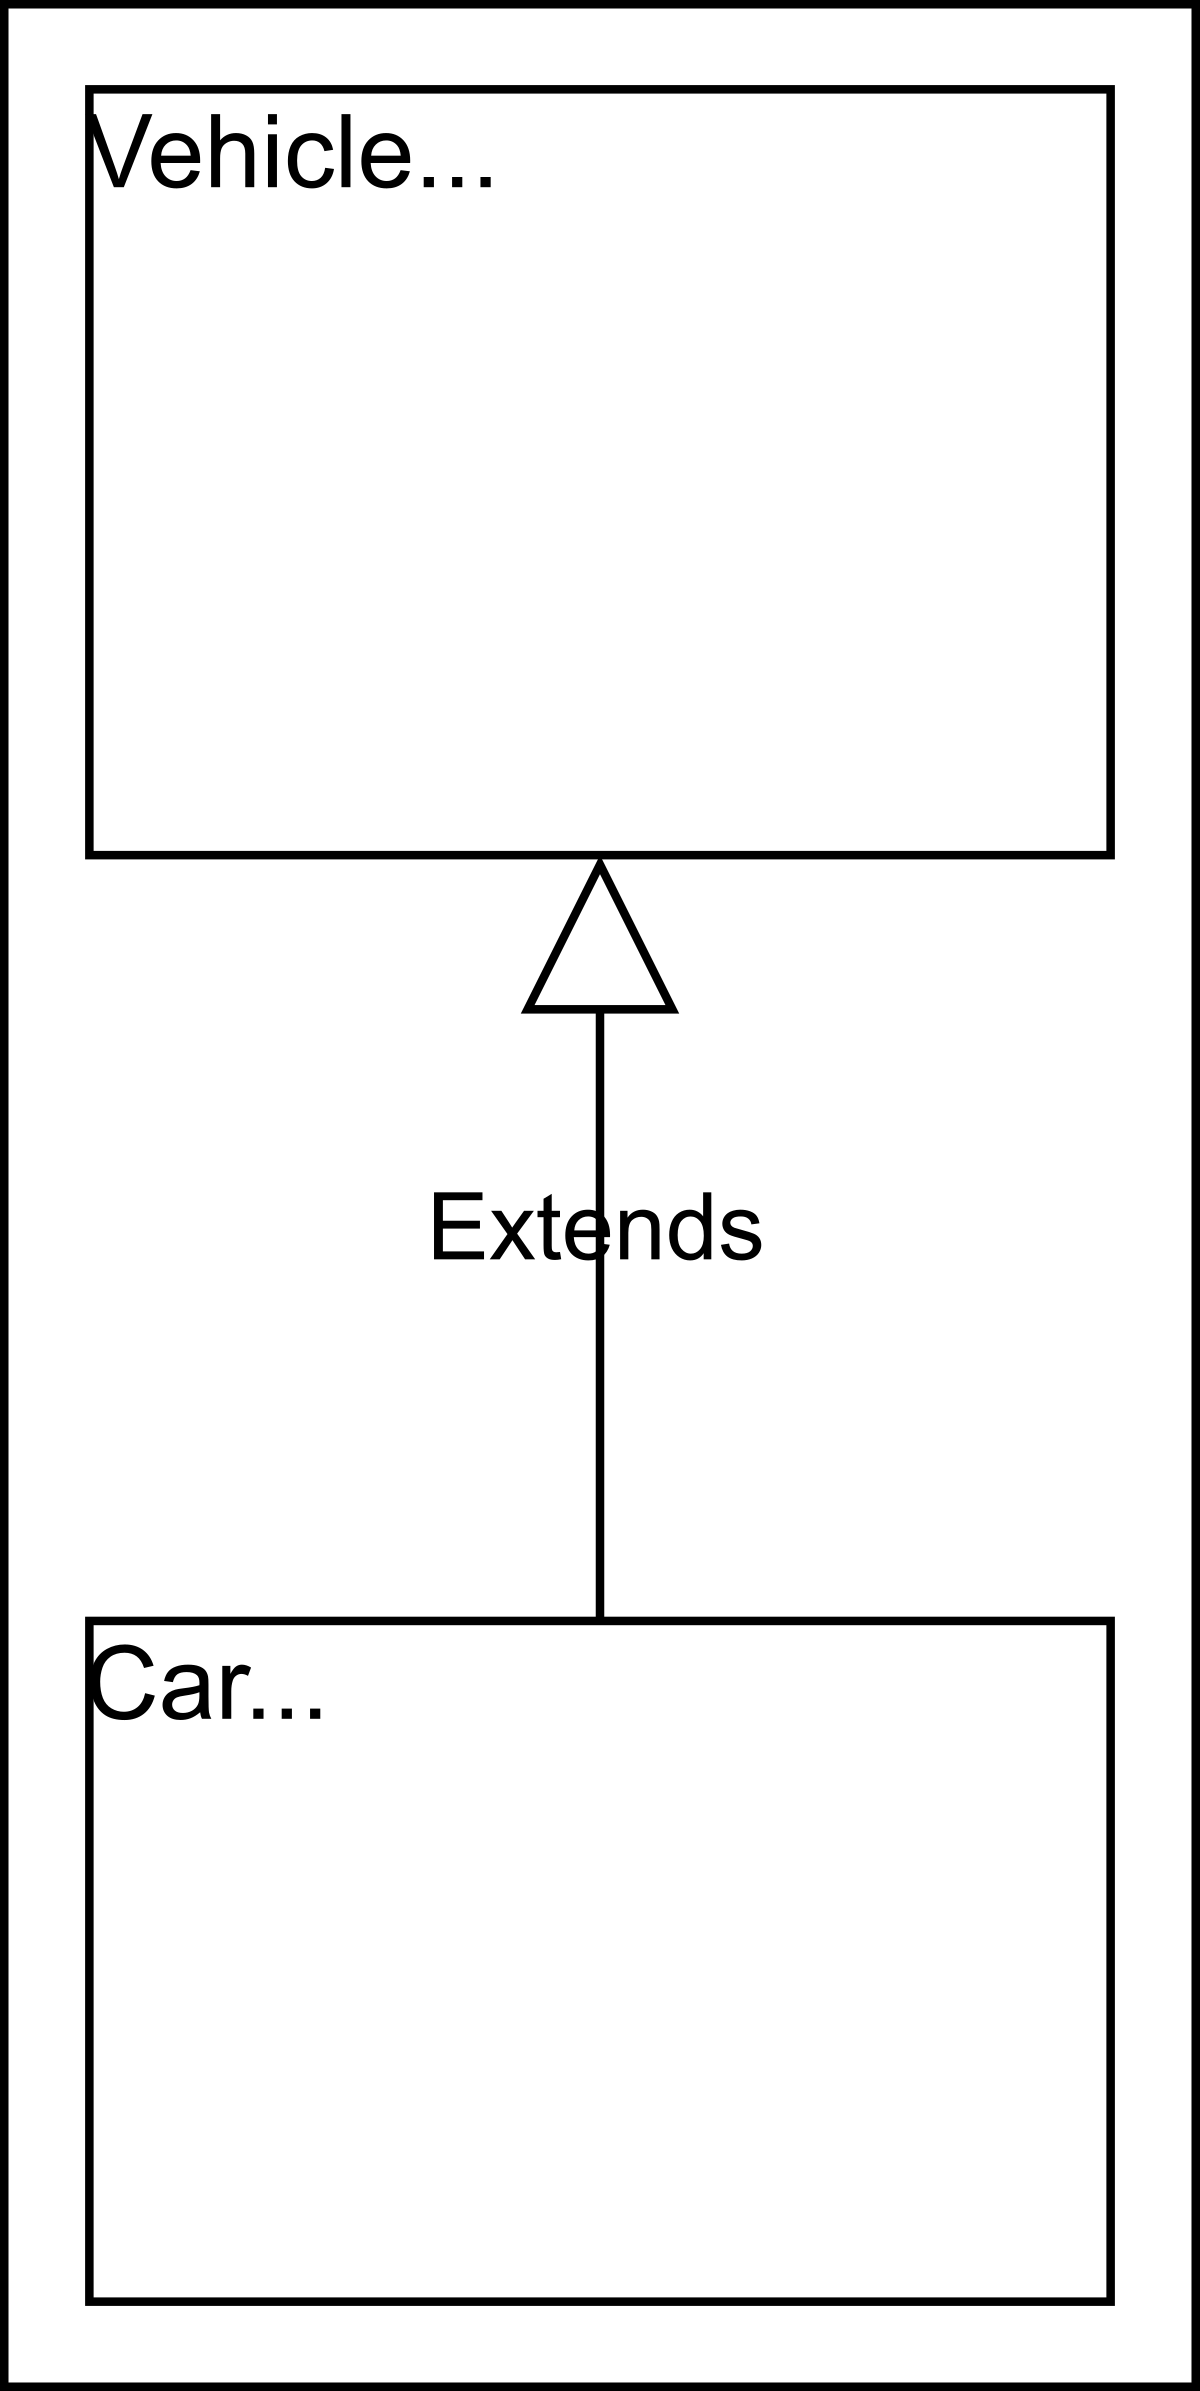
\includegraphics[width=0.5\textwidth]{Images/chapter_4/section_4941477451137024/5519108160618496.png}
 \caption{The vehicle superclass}
\end{figure}

So far, this implementation seems right since a car IS A vehicle, and the \texttt{startEngine()} method will override the superclass method. However, it\textquotesingle s not as simple as it looks.

\subsubsection{Violation}\label{violation}
\\
Let\textquotesingle s add a \texttt{Bicycle} subclass in this system and see what happens:

\begin{figure}[htbp]
 \centering
 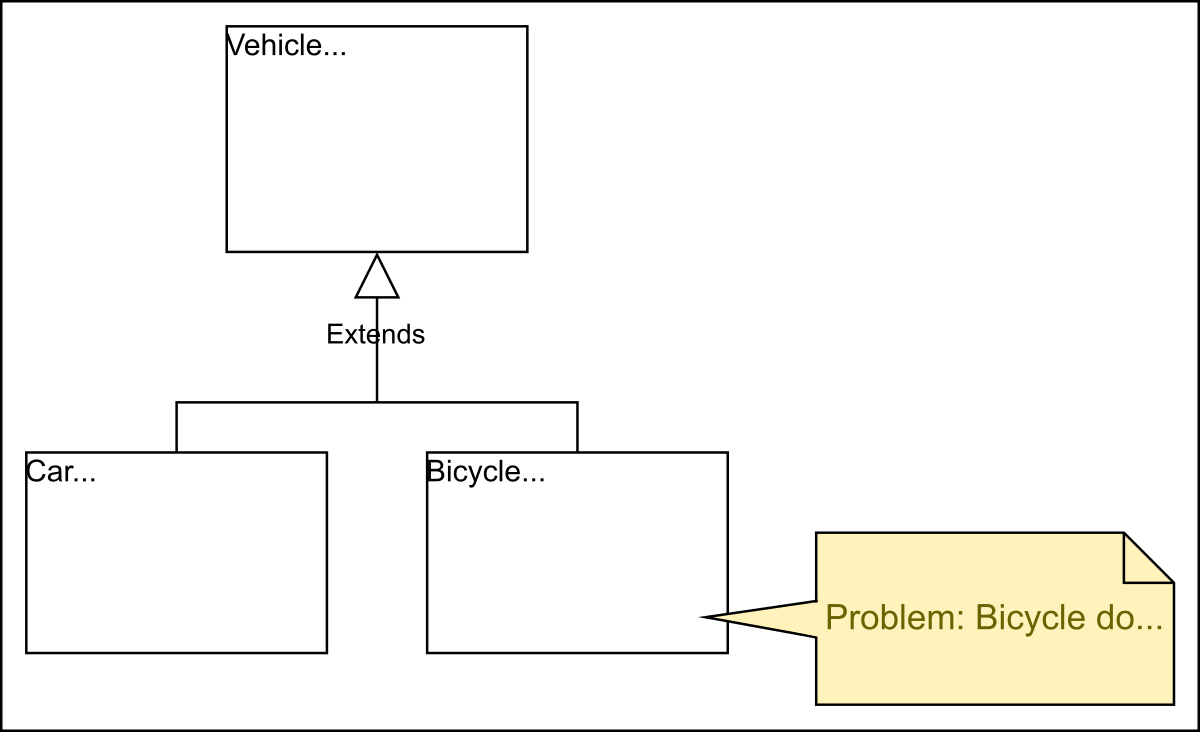
\includegraphics[width=0.5\textwidth]{Images/chapter_4/section_4941477451137024/4522889232777216.png}
 \caption{Violation of the LSP}
\end{figure}

This results in a problem. A bicycle is a vehicle, but it does not have an engine. Therefore, the \texttt{Bicycle} class should not be allowed to override the \texttt{startEngine()} method.

\subsubsection{Solution}\label{solution}
\\
A possible fix to this issue would be to add two subclasses of \texttt{Vehicle} that classify the vehicles as motorized vehicles and manual vehicles as follows:

\begin{figure}[htbp]
 \centering
 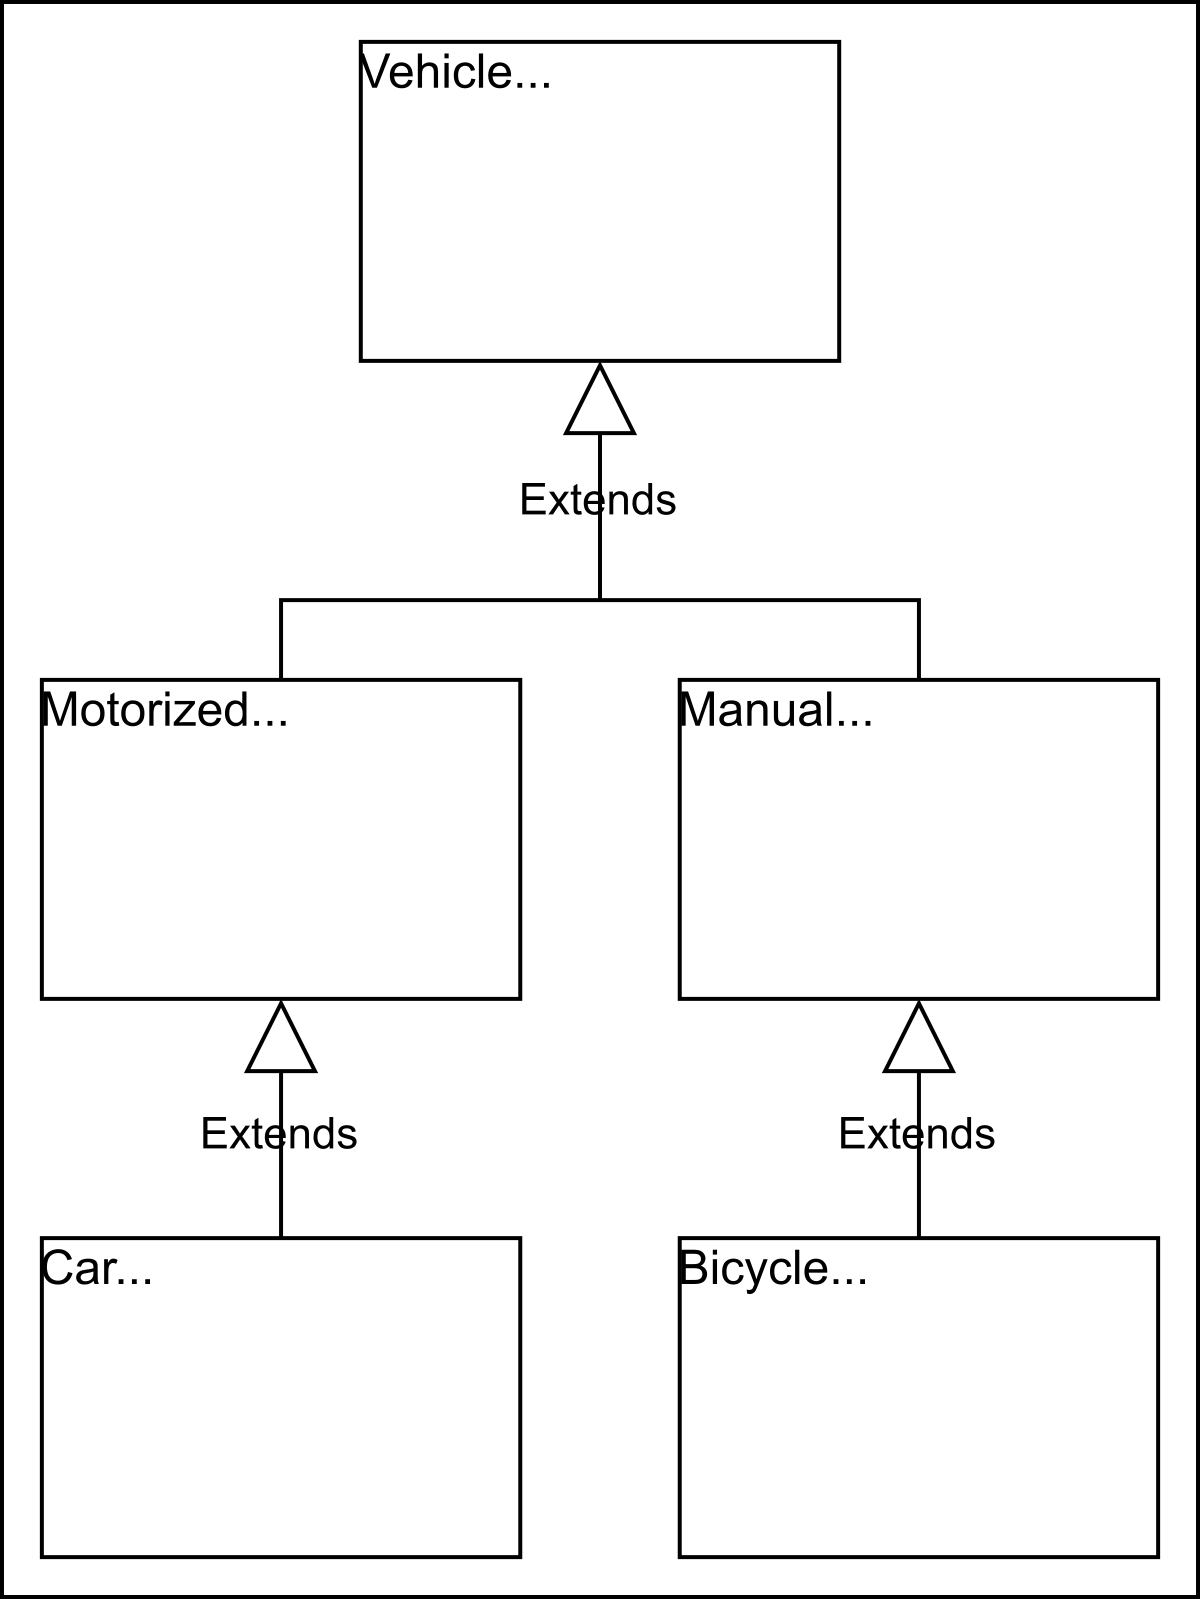
\includegraphics[width=0.5\textwidth]{Images/chapter_4/section_4941477451137024/5276869583962112.png}
 \caption{An example of the LSP implementation}
\end{figure}

With this implementation, we have satisfied the LSP.

\begin{itemize}
\item
\texttt{Car} is substitutable with its superclass, \texttt{Motorized}, and \texttt{Bicycle} is substitutable with its superclass, \texttt{Manual}, without breaking the functionality.
\item
Their methods can also override the methods of the superclass.
\end{itemize}

\subsection{Conclusion}\label{conclusion}
\\
The LSP is an important principle that should be extended to the level of system architecture. A small violation of the substitutability of classes can cause the system to break down, which is why we should always be on the lookout for violations. A few benefits of the LSP are provided below:

\begin{itemize}
\item
It avoids the generalization of concepts that may not be needed in the future.
\item
It makes the code maintainable and easier to upgrade.
\end{itemize}
\\
Now that we have learned about the Liskov Substitution Principle, let\textquotesingle s look at the Interface Segregation Principle in the next lesson.

% End of section content